\section{EXPLORATION AND MAPPING OVERVIEW}
%\section{EXPLORATION STRATEGY DESCRIPTION}
%Change the title--Method overview
The laser scan and odometry sensor measurements of the mobile robot represent input data for a Simultaneous Localisation and Mapping (SLAM) module. In this work, for map building we use a submap-based graph SLAM method -- Google Cartographer \cite{Hess2016} -- which, however, in the simulation uses the ground truth mobile robot poses (\textit {perfect localisation}) from the Stage simulator \cite{stageweb} in order to eliminate the SLAM algorithm uncertainty. The module also implements frontier detection according to \cite{Orsulic2019}. This method has achieved impressive results in terms of wall-time per frontier update, what greatly speeds up our exploration and mapping process. 

Google Cartographer SLAM extended with frontier detection and filter module are centralized part of the exploration and mapping process (Fig. \ref{fig:exploration-strategy}). Centralized part generates filtered frontier points, inputs to $n$ equal decentralized strategies modules for $n$ mobile robots. During the exploration and mapping $n$ mobile robots communicate, exchange minimum information about frontier points in order to decide where to navigate and create common map of the unknown environment. Focus and scope of the paper is decentralization of the decision making process, using centralized SLAM algorithm and centralized filtered frontier point generator. Further, the algorithm for path planning and following navigates the mobile robot toward the target point. The process is over when the area is explored.  

\begin{figure}[t!]
    \centering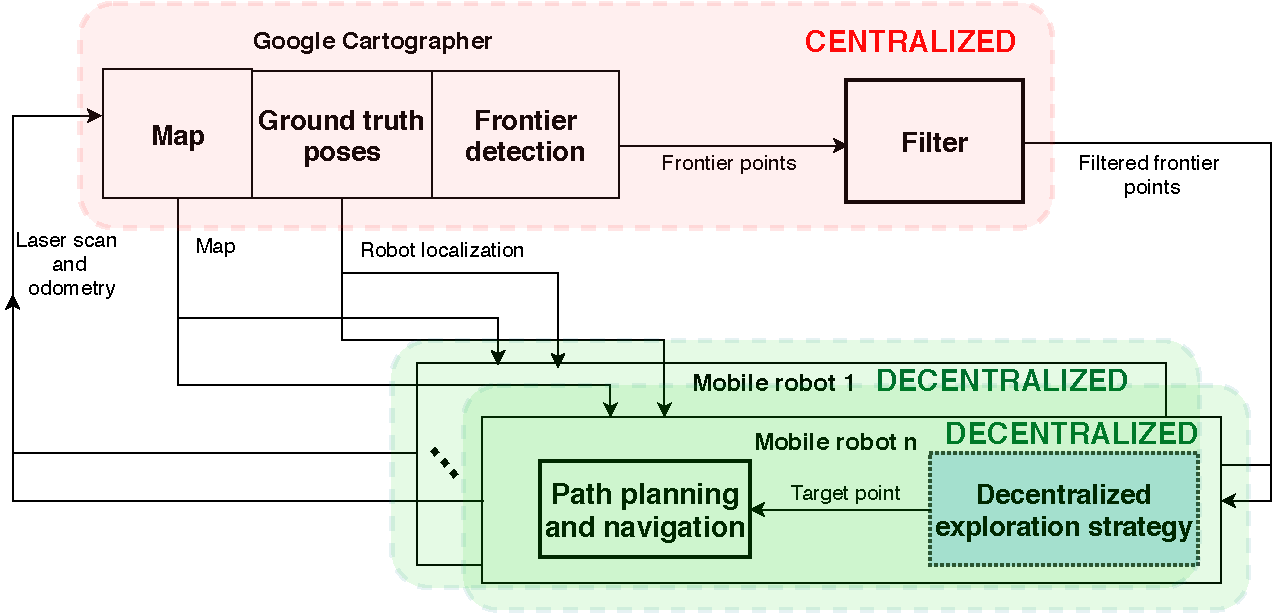
\includegraphics[width=1.0\columnwidth]{./Pictures/diagram_exploration.pdf}
	\caption{Overall schematic diagram of the decentralized exploration and mapping process for $n$ mobile robots in the simulator. Google Cartographer and filter module (highlighted red) generate filtered frontier points that are centralized part of exploration and mapping process. Exploration strategy and path planning and navigation module (highlighted green) are decentralized parts that generate $n$ outputs and create common map.}
   \label{fig:exploration-strategy}
\end{figure}

Our multi-robot exploration and mapping process combine SLAM (Google Cartographer), a frontier detection algorithm, filter module and a decision making strategy. Each component can be easily changed or extended, without affecting an exploration and mapping process. For instance, the decentralized strategy can be replaced without affecting the frontier points detection. Similarly different types of frontier points detectors could be tested without affecting the behaviour of the decision making strategy. The same logic is valid for SLAM method and filter module. This makes our exploration and mapping process more flexible and modular. 

\subsection{SLAM} 
Most literature uses the ROS 'gmapping' package for generating the
map and localizing mobile robots \cite{Keidar2012}, \cite{Umari2017}. The 'gmapping' package implements a SLAM algorithm that uses a Rao-Blackwellized particle filter \cite{Grisetti2007}. 
On the other side, we use Google Cartographer SLAM algorithm \cite{Hess2016}, an open source available in \cite{cartographer}, which in our case generates ground truth map. Cartographer is an open-source 2D and 3D graph SLAM based on occupancy grid submaps. 
An extension to the Cartographer is a new fast frontier detection method developed in \cite{Orsulic2019}. 

\subsection{Frontier Detection}
A popular frontier-based exploration approach is introduced by Yamauchi \cite{Yamauchi1998}, where the robots explore an unknown environment and build a common map. Moreover, each robot heads to the center of mass of the closest frontier and frontier detection is performed only when the robot reaches its target. 
The frontier edges detection can be achieved using RRT (Rapidly Exploring Random Tree) algorithm by Umari and Mukhopadhyay \cite{Umari2017}. The RRT algorithm is biased towards unexplored regions and provides a general approach which can be extended to higher dimensional spaces. However, RRT algorithm proved not to be fast enough in instances when larger parts of the environments were explored, so we opted to use a dense frontier detection method \cite{Orsulic2019}. Orsulic has achieved great results in terms of wall-time per frontier update. Furthermore, this paper is the first usage of the dense frontier detection method in multi-robot exploration and mapping. 

\subsection{Filter Module}

The filter module receives the frontier points from frontier detector  and first clusters the points and stores only the centre of each cluster. The clustering process reduce the number of frontier points from frontier detection module, which are extremely close to each other. If such amount of points are sent to the decentralized exploration strategy module, there would be unnecessary consumption of computational resources, without additional information about the frontier. We use Hierarchical Agglomerative Clustering \cite{clutering} because it does not require predefined number of clusters. We only need to set distance threshold parameter, above which clusters will not be merged. Even though it has a time complexity of ${\displaystyle {\mathcal {O}}(n^{3})}$, it is suitable for our case because of the size of frontier points. Moreover, it is easy to implement. 

\subsection{Why Decentralized?}

Algorithms for assigning robots to target points can be grouped into centralized and decentralized algorithms. Centralized task assignment for a multi-robot system may be less practical due to communication limits \cite{Dias2000}, robustness issues \cite{Dias2006}, or time required for algorithm execution and scalability \cite{Julia2012}. In the centralized approach, each mobile robot receives tasks assigned from a single central \emph{leader} using a centralized planning algorithm. During communication between the central leader and the mobile robots, information about the mobile robot poses is shared in order to perform real time mobile robot task allocation. The central leader may be a computer or a robot. An advantage of centralized approach is that the optimal plans can be found \cite{Yan2011}. Nevertheless, this mechanism is ineffectual for large mobile robot teams.

In contrast to centralized approaches, in a decentralized approach, the mobile robots are completely autonomous in the exploration process. Each mobile robot has its own local knowledge of the world and can decide its future actions by taking into account its current context and task, its own capacities and the capacities of the other mobile robots, through a negotiation process \cite{Yan2013}. Moreover, it usually has better reliability, flexibility, adaptability and robustness \cite{Zlot2002}. There is no central planner in the decentralized multi-robot exploration problem, so mobile robots need to communicate and cooperate effectively to explore and map an unknown environment as soon as possible. 
In order to have more robust and flexible system we propose a strategy in which mobile robots are able to decide toward which target point to navigate, with the assumption that the mobile robots have knowledge of all target points, while we assume that only a single mobile robot can be assigned to a specific target point.  

In this paper we determine the target points for each mobile robot in the team using an objective function which is a combination of frontier point cost, utility of reaching the target point and a novel extension - the frontier occupancy function that makes mobile robot be dispersed throughout the environment. 
